\section{Measuruments in Qiskit}

Measuring the outcome of the qubits in a Quantum circuit is very important in Quantum Computing because it allows us to verify our
algorithm quantitativily. Qiskit allows us to measure in two ways: measure a qubit into a specific bit or measure every qubit at once
into a classical register.

If we want to measure each qubit or group of qubit into specific bits or classical registers we must ensure to instanciate the circuit
object with the appropriate amount of bits. This can be done by passing an integer as the second parameter on instanciation. Then
we can specify which qubit line we want to measure into which bit line by invoking the \verb|measure()| member method of the circuit
object.

\begin{figure}[ht]
    \centering
    \begin{minted}{python3}
        from qiskit import QuantumCircuit

        circuit = QuantumCircuit(2, 2) # 2 qubits + 2 bits
        
        circuit.h(0)
        circuit.x(1)

        circuit.measure(0, 0) # measure q_0 and store the outcome on c_0
        circuit.measure(1, 1) # measure q_1 and store the outcome on c_1

        print(circuit.draw("latex_source"))
    \end{minted}
    \centering
    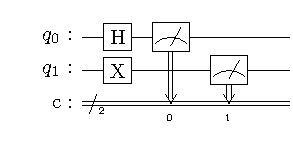
\includegraphics{images/4_Qiskit/example_meas_q2b_1.pdf}
    \caption{Measuring qubit states into the appropriate bits}
\end{figure}

Finally, if we want to measure all qubits at once we can invoke the \verb|measure_all()| member method of the circuit object.
Note that we do not need to specify how many bits the cirucit needs, Qiskit auto-calculates the appropriate amount and
supplies the circuit with a pre-allocated classical register named \verb|meas|.

\begin{figure}[ht]
    \begin{minted}{python3}
        from qiskit import QuantumCircuit
    
        circuit = QuantumCircuit(2, 2)
        
        circuit.h(0)
        circuit.x(1)
    
        circuit.measure_all() # measure everything in one batch
    
        print(circuit.draw("latex_source"))
    \end{minted}
    \centering
    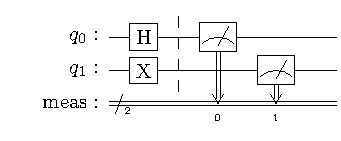
\includegraphics{images/4_Qiskit/example_meas_all_1.pdf}
    \caption{Measuring all the qubit outcomes of the circuit at once}
\end{figure}